\documentclass{homework}

\title{Homework 7}
\author{Kevin Evans}
\studentid{11571810}
\date{March 25, 2021}
\setclass{Physics}{465}
\usepackage{amssymb}
\usepackage{mathtools}
\usepackage{amsthm}
\usepackage{amsmath}
\usepackage{physics}
\usepackage{booktabs}
\usepackage{multirow}
\usepackage[inter-unit-product =\cdot]{siunitx}

\usepackage{times}
\usepackage{mhchem}
\usepackage{tikz}

\usepackage[compat=1.1.0]{tikz-feynman}
%\usepackage{calligra}
%\DeclareMathAlphabet{\mathcalligra}{T1}{calligra}{m}{n}
%\DeclareFontShape{T1}{calligra}{m}{n}{<->s*[2.2]callig15}{}
%\newcommand{\scriptr}{\mathcalligra{r}\,}
%\newcommand{\boldscriptr}{\pmb{\mathcalligra{r}}\,}
%\newcommand{\emf}{\mathcal{E}}

\DeclareSIUnit\eVperc{\eV\per\clight}
\DeclareSIUnit\clight{\text{\ensuremath{c}}}
\DeclareSIUnit\year{yr}
\newcommand{\M}{\ensuremath{\mathcal{M}}}
\newcommand{\fm}{\femto\meter}

\renewcommand{\P}{\ensuremath{\mathbb{P}}}

\newcommand{\solution}{	\vspace{1em} \textit{Solution.} \quad }

\begin{document}
	\maketitle
	\begin{enumerate}
		\item[9.1] % 9.1
			Show that the gauge transformation of the equations (9.3) leave unchanged the magnetic and electric field equations (9.1) and (9.2).
			
			\solution From the gauge transformations of (9.3), \begin{align*}
				\bvec{A} \to \bvec{A}' & = \bvec{A} + \grad \Lambda \\
				\varphi \to \varphi' & = \phi - \pdv{\Lambda}{t},
				\intertext{We can apply these to the fields of (9.1) and (9.2),}
				\bvec{B}' & = \curl \bvec{A}' \tag{9.1} \\
					& = \curl[\bvec{A} + \grad{\Lambda}] \\
					& = \curl{\bvec{A}} + \underbrace{\curl[\grad{\Lambda}]}_{0} && \text{(curl of a grad.)} \\
					& = \curl{\bvec{A}} = \bvec{B}. \qed \\
				\bvec{E}' & = -\grad{\phi'} - \pdv{\bvec{A}'}{t} \tag{9.2} \\
					& = - \grad{\phi} + \grad{\pdv{\Lambda}{t}} - \pdv{\bvec{A}}{t} - \pdv{t}[\grad{\Lambda}] \\
					& = -\grad{\phi} - \pdv{\bvec{A}}{t} = \bvec{E}. \qed && \text{(linearity)}
			\end{align*}
		
		\item[9.2] % 9.2
			Show that the processes represented by Fig. 9.2(a)--(d) cannot satisfy the rule that energy and momentum are conserved at a vertex if all three particles in each case are free. (This means that all of these processes are physically impossible under that condition.)
			
			\solution Looking at each of these processes on p. 161, \begin{enumerate}
				\item Photon emission by an electron. Here, the photon emission must be caused by an accelerating charge. This would mean the outgoing electron has more energy than the initial stationary electron. Therefore this violates \underline{conservation of energy.}
				
				\item Photon absorption by an electron. % must be bound?
					This violates \underline{conservation of energy}, as the incoming photon and electron pair must have greater energy (as they both have a momentum) than a single electron with no momentum.
				
				\item Photon emission by a positron. This violates \underline{conservation of momentum}, as the outgoing electron-positron pair has a CM frame with $\bvec{p}=0$, but the incident photon must not have a zero momentum.
				
				\item Photon materialization into an electron-position pair. This violates \underline{conservation of momentum}. There exists a center of momentum frame such that the outgoing \ce{e^-} and \ce{e^+} have a net $\bvec{p}=0$, however the incoming photon cannot have a zero momentum.
			\end{enumerate}
			
		\pagebreak
		
		\item[9.3] % 9.3
			Find the two leading-order diagrams for electron-electron elastic scattering. (The two to be found are both two-vertex diagrams.) Find one and label all the in-going and out-going particles with type and four-momentum. Then find a second which is different; note that there can be no annihilation diagram like that of Fig 9.3(b).
			
			\solution
			
			\hfil
			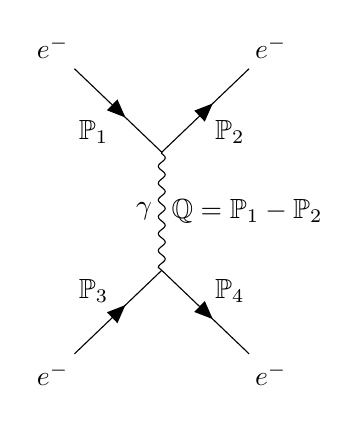
\begin{tikzpicture}[baseline=(current  bounding  box.north west)]
				\begin{feynman}
					\vertex (a);
					\vertex [above left=of a](e1){$e^-$};
					\vertex [above right=of a](e2) {$e^-$};
					\vertex [below=of a] (b);
					\vertex [below left=of b](e3){$e^-$};
					\vertex [below right=of b](e4){$e^-$};
					\diagram* {
						(e1) -- [fermion,edge label'={$\P_1$}] (a) -- [fermion, edge label'={$\P_2$}] (e2),
						(a) -- [boson,edge label'=$\gamma$,edge label={$\mathbb{Q}=\P_1 - \P_2$}] (b),
						(e3) -- [fermion, edge label=$\P_3$] (b) -- [fermion, edge label=$\P_4$] (e4)
					};
				\end{feynman}
			\end{tikzpicture}
			\hfil
			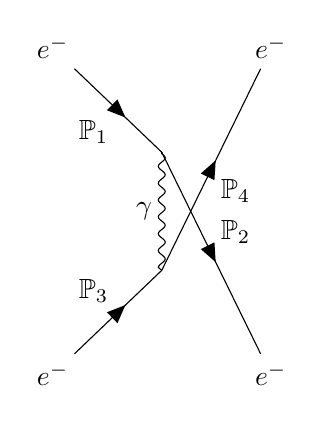
\begin{tikzpicture}[baseline=(current  bounding  box.north west)]
				\begin{feynman}
					\vertex (a);
					\vertex [above left=of a](e1){$e^-$};
					\vertex [above right=of a](e2) {$e^-$};
					\vertex [below=of a] (b);
					\vertex [below left=of b](e3){$e^-$};
					\vertex [below right=of b](e4){$e^-$};
					\diagram* {
						(e1) -- [fermion,edge label'={$\P_1$}] (a),
						(b)  -- [fermion, edge label'={$\P_4$}] (e2),
						(a) -- [boson,edge label'=$\gamma$] (b),
						(e3) -- [fermion, edge label=$\P_3$] (b),
						(a)  -- [fermion, edge label=$\P_2$] (e4)
					};
				\end{feynman}
			\end{tikzpicture}
			\hfil
			
			\vspace{2em}
			
		\item[9.4] % 9.4
			Find the two leading-order diagrams for the production of an electron-positron pair by a real photon in the electric field of the nucleus.
			
			\solution 
			
			%%%%%%% I think the second diagram uses the nucleus photon to generate the virtual particle instead of the incident ray
			\hfil
			\begin{tikzpicture}
				\begin{feynman}
					\vertex (a);
					\vertex [left=of a] (g1) {$\gamma$};
					\vertex [above right=of a] (e1) {$e^+$}; 
					\vertex [below right={3 em} of a](b);
					\vertex [below left=of b](z){$Z$};
					\vertex [below right=of b](e2) {$e^-$};
					\diagram* {
						(g1) -- [boson] (a),
						(e1) -- [fermion] (a) -- [fermion, edge label=$e^-$] (b) -- [fermion] (e2),
						(z) -- [boson, edge label=$\gamma$] (b)
					};
				\end{feynman}
			\end{tikzpicture}
			\hfil
			\begin{tikzpicture}
				\begin{feynman}
					\vertex (a);
					\vertex [left=of a] (g1) {$Z$};
					\vertex [above right=of a] (e1) {$e^+$};
					\vertex [below right={3 em} of a](b);
					\vertex [below left=of b](z){$\gamma$};
					\vertex [below right=of b](e2) {$e^-$};
					\diagram*{
						(g1) -- [boson, edge label=$\gamma$] (a),
						(e1) -- [fermion] (a) -- [fermion, edge label=$e^-$] (b) -- [fermion] (e2),
						(z) -- [boson] (b)
					};
				\end{feynman}
			\end{tikzpicture}
			\hfil
			
			\pagebreak
			
		\item[9.5] % 9.5
			Consider a system consisting of two non-identical spin-$\frac{1}{2}$ fermions: list all the allowed states that are simultaneously eigenstates of the operators $L^2$, $S^2$, $J^2$ up to $\ell=3$ by their spectroscopic notation. For each value of $j_P$, where $P$ is the parity, and the symmetry. Check that \ce{^3 D_1} and \ce{^3 S_1} are the only states with $j_P=1^+$.
			
			All the states that have you listed are available to the neutron-proton system, but only half are available to the neutron-neutron and proton-proton systems: list these.
			
			\solution 
			$$
				\begin{array}{clcc}
					\toprule
					L & \text{State} & J & \text{Exchange Sym.} \\
					\midrule
					\multirow{2}{*}{$L=0$} & \ce{^1 S_0} & 0^+ & a \\
						& \ce{^3 S_1} & 1^+ & s \\
					\midrule
					\multirow{4}{*}{$L=1$} & \ce{^1 P_1} & 1^- & s \\
						& \ce{^3 P_0} & 0^- & a \\
						& \ce{^3 P_1} & 1^- & a \\
						& \ce{^3 P_2} & 2^- & a \\
					\midrule
					% L=2
					% S=0 => J=2
					% S=1 => J=3, J=2, J=1
					\multirow{4}{*}{$L=2$} & \ce{^1 D_2} & 2^+ & a \\
					& \ce{^3 D_3} & 3^+ & s  \\
					& \ce{^3 D_2} & 2^+ & s \\
					& \ce{^3 D_1} & 1^+ & s \\
					\midrule
					% L=3
					% S=0 => J=3
					% S=1 => J=4, 3, 2
					\multirow{4}{*}{$L=3$} & \ce{^1 F_3} & 3^- & s\\
					& \ce{^3 F_4} &  4^- & a\\
					& \ce{^3 F_3} & 3^- & a\\
					& \ce{^3 F_2} & 2^- & a\\
					\bottomrule
				\end{array}
			$$
			For a n-n and p-p system, only the antisymmetric ($a$) states area available due to the Pauli principle.
		\pagebreak
		
		\item[6.] Yukawa hypothesis and derivation, following Table 9.5.
			
			\solution To begin, we can consider the relativistic energy-momentum relation, $$E^2 - \bvec{P}^2 c^2 = m^2 c^4.$$
			Using the energy and momentum operators, \begin{align*}
				\hat{E} & = +i \hbar \pdv{t} \\
				\hat{\bvec{P}} & = - i \hbar \grad,
			\end{align*}
			the energy-momentum relation for a wavefunction $\Psi$ becomes \begin{equation*}
					-\hbar^2 \pdv[2]{\Psi}{t} + \hbar^2 c^2 \laplacian{\Psi} = m^2 c^4 \Psi. \label{ep} \tag{$*$} 
			\end{equation*}
			In the static case, we assume $$\pdv{\Psi}{t} = 0,$$
			then \eqref{ep} reduces to $$\laplacian{\Psi} = \left(\frac{mc}{\hbar}\right)^2 \Psi.$$
			This has solutions of the form $$\Psi = (1/r) \exp(-\frac{mc}{\hbar}r).$$
			The points towards a potential with a range of roughly $$\text{range} \quad a  = \hbar / m c.$$
	\end{enumerate}
\end{document}